\chapterhead{6}{Finding Missing Energy}{Spotting a gap, and a diagram that cheats}\label{ch6}

An energy account has a rule: what comes out adds up to what went in. When a number is short, the gap needs a name, such as warmth or sound. When a number is \emph{too big}, something is wrong, because energy cannot appear from nowhere. A good account checks both.

\begin{center}
\sffamily\small\renewcommand{\arraystretch}{1.5}
\begin{tabular}{@{}p{3.4cm}p{3.7cm}p{3.7cm}@{}}
\toprule
\textbf{Model} & \textbf{What it keeps} & \textbf{What it drops}\\
\midrule
Energy as heights & the stored energy of a ball & its weight and shape\\
A roll or a cooling & what moved or left & where the warmth ended up\\
A machine as a trade & less force for more distance & what is inside\\
An energy ledger & where the loss happened & the cause of the loss\\
\bottomrule
\end{tabular}
\end{center}

\begin{tryit}{Expected against found}
Drop from 40. Use the rule from chapter~1: each bounce gives back about 7 tenths. Expected heights are about 28, 20 and 14. Measure the real bounces and compare. Does any bounce lose more than expected?\par\medskip
\renewcommand{\arraystretch}{1.6}
\begin{tabular}{|l|c|c|c|}
\hline
\textbf{Bounce} & \textbf{Expected} & \textbf{Found} & \textbf{Extra lost}\\ \hline
1 & 28 & & \\ \hline
2 & 20 & & \\ \hline
3 & 14 & & \\ \hline
\end{tabular}
\end{tryit}

\begin{worked}{Practice numbers, not from a real test}
Found: 28, 20, 10. Extra lost: 0, 0 and $14-10=4$.\\
The gap appeared at bounce 3. The ball had clipped a chair leg and thumped it, so the extra 4 units went into the chair and into sound.
\end{worked}

\begin{center}
\sffamily\small\renewcommand{\arraystretch}{1.5}
\begin{tabular}{@{}lrrr@{}}
\toprule
\textbf{Bounce} & \textbf{Expected} & \textbf{Found} & \textbf{Extra lost}\\
\midrule
1 & 28 & 28 & 0\\
2 & 20 & 20 & 0\\
3 & 14 & 10 & \textbf{4}\\
\bottomrule
\end{tabular}
\end{center}

\begin{multix}[hmm]\multixbot[hmm]\tcblower
Four units were short at bounce 3, so four units were destroyed. I wrote ``destroyed'' in the ledger. Neat. Is it?
\end{multix}

\trust{We compared what the bounce rule expected with what we found at every bounce, so the step with the gap was visible.}
{Only bounce 3 showed extra loss, and the chair leg matched it.}
{That every gap has such a visible cause. Gaps of 1 or 2~cm are within our reading error and cannot be traced.}

\begin{keepbox}
We turned an energy account into expected and found. \textbf{We kept} \wline[3.4cm] \textbf{and we set aside} \wline[3.4cm].
\end{keepbox}

\clearpage

\subhead{Spot the diagram that cheats}
Here are four claims, each drawn as circles. Three balance, or have a named gap. One makes energy from nowhere.

\begin{center}
\begin{tikzpicture}[scale=0.95]
  % A
  \node[font=\sffamily\bfseries\small] at (0,3.3) {A: ball bounce};
  \node[bigcir,minimum size=1.6cm] (a1) at (0,1.8) {}; \node[font=\sffamily\scriptsize] at (0,1.8) {drop 40};
  \node[cir,inner sep=1pt] (a2) at (2.7,2.4) {28}; \node[cir,inner sep=1pt] (a3) at (2.7,1.2) {12};
  \draw[popA] (a1) -- (a2); \draw[popA] (a1) -- (a3);
  % B
  \node[font=\sffamily\bfseries\small] at (6.4,3.3) {B: ball bounce};
  \node[bigcir,minimum size=1.6cm] (b1) at (6.4,1.8) {}; \node[font=\sffamily\scriptsize] at (6.4,1.8) {drop 40};
  \node[cir,inner sep=1pt] (b2) at (9.1,1.8) {46};
  \draw[popA] (b1) -- (b2);
  % C
  \node[font=\sffamily\bfseries\small] at (0,-0.6) {C: pulley};
  \node[bigcir,minimum size=1.6cm] (c1) at (0,-2.0) {}; \node[font=\sffamily\scriptsize] at (0,-2.0) {pull 64};
  \node[cir,inner sep=1pt] (c2) at (2.7,-1.4) {60}; \node[cir,inner sep=1pt] (c3) at (2.7,-2.6) {4};
  \draw[popA] (c1) -- (c2); \draw[popA] (c1) -- (c3);
  % D
  \node[font=\sffamily\bfseries\small] at (6.4,-0.6) {D: rolling ball};
  \node[bigcir,minimum size=1.6cm] (d1) at (6.4,-2.0) {}; \node[font=\sffamily\scriptsize] at (6.4,-2.0) {ramp 20};
  \node[cir,inner sep=1pt] (d2) at (9.1,-1.4) {20}; \node[cir,inner sep=1pt] (d3) at (9.1,-2.6) {0};
  \draw[popA] (d1) -- (d2); \draw[popA] (d1) -- (d3);
\end{tikzpicture}
\end{center}

Which diagram cheats? \wline[1.6cm] How many units appeared from nowhere? \wline[1.6cm]\\[8pt]
Which diagram has a gap that is named? \wline[1.6cm] What is the name? \wline[3cm]

\clearpage

\begin{puzzle}{Find the step}
Start 60. After step 1 expected 42, found 42. After step 2 expected 29, found 24. Which step lost extra? \wline[1.6cm] How much? \wline[1.6cm]
\end{puzzle}

\begin{puzzle}{Too good}
A ball dropped from 30 bounced to 36. Does it break the account? \wline[2cm] Name one thing that might have gone wrong. \wline[4cm]
\end{puzzle}

\begin{puzzle}{Lever check}
3 coins at 10~cm are said to balance 2 coins at 10~cm. Do the products match? \wline[2cm]
\end{puzzle}

\begin{puzzle}{Within error?}
A bounce was found 1~cm lower than expected, and heights are read to about 1~cm. Can you tell where it went? \wline[2cm] Why? \wline[4cm]
\end{puzzle}

\begin{puzzle}{Check one step}
Why is checking after every bounce better than checking only the last one? \wline[6cm]
\end{puzzle}

\clearpage

\begin{puzzle}{Add the gaps}
Extra losses of 0, 2 and 1 at three steps. Total \wline[1.6cm]
\end{puzzle}

\begin{puzzle}{Model or real?}
Write M for model and R for real thing.\\
(a) a circle with 28 in it \wline[1cm] \quad (b) the bouncing ball \wline[1cm] \quad (c) a table of heights \wline[1cm]
\end{puzzle}

\begin{puzzle}{Which question?}
The ledger can answer ``where did the energy go?'' Can it answer ``why did the ball clip the chair?'' \wline[2cm] What else would you need? \wline[4cm]
\end{puzzle}

\begin{puzzle}{Unfair ledger}
Ana measured bounces on a rug and Ben on a bare floor, and then they added their losses. Why does that mislead? \wline[6cm]
\end{puzzle}

\clearpage

\begin{puzzle}{Recount}
Bounces from 40 were 28, 20 and 10. Losses were 12, 8 and \wline[1.2cm]. Total lost \wline[1.2cm]
\end{puzzle}

\begin{puzzle}{Wrap}
A student wrote ``4 units were destroyed.'' Wrap it with a better claim. \wline[6cm]
\end{puzzle}

\begin{puzzle}{A good habit}
Write one habit from this book that makes an energy account more trustworthy. \wline[6cm]
\end{puzzle}

\begin{puzzle}{Missing step}
A student measured only the drop and the last bounce, then said all of the loss was ``warmth''. What could go wrong? \wline[6cm]
\end{puzzle}

\clearpage

\begin{puzzle}{Draw the step circles}
Draw a bounce as circles: a drop of 40, a bounce of 28 and the loss.
\begin{center}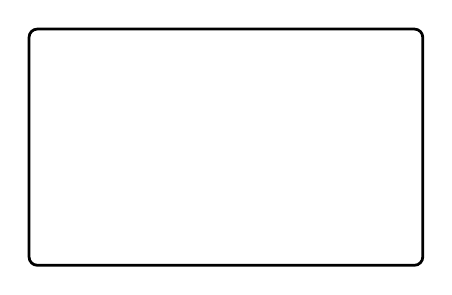
\begin{tikzpicture}\draw[line width=1pt,rounded corners=3pt] (0,0) rectangle (5,3); \end{tikzpicture}\end{center}
\end{puzzle}

\begin{puzzle}{Draw the gap}
Draw bounce 3 with its 4 unit extra loss as its own circle.
\begin{center}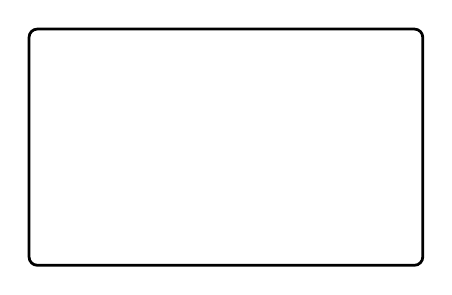
\begin{tikzpicture}\draw[line width=1pt,rounded corners=3pt] (0,0) rectangle (5,3); \end{tikzpicture}\end{center}
\end{puzzle}

\begin{puzzle}{Draw the wrap}
Draw a circle around ``4 units destroyed'' and write the corrected claim outside it.
\begin{center}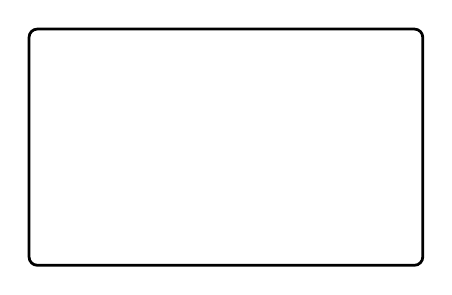
\begin{tikzpicture}\draw[line width=1pt,rounded corners=3pt] (0,0) rectangle (5,3); \end{tikzpicture}\end{center}
\end{puzzle}

\clearpage
\thispagestyle{fancy}\label{slop}
\subhead{Slop check}
Slop is hasty, gaudy work that forgot to take care. It can be made by a person or a machine, quickly or slowly. What matters is whether the work shows care for three things:
\begin{itemize}[leftmargin=1.6em]
\item \textbf{Salient:} Is the main point easy to see?
\item \textbf{Simple:} Is there anything that does nothing but get in the way?
\item \textbf{Relevant:} Does everything on the page help answer the question?
\end{itemize}

Here is a hasty poster about a bouncing ball. Study it, then decide what is wrong.

\begin{center}
\begin{tikzpicture}[scale=0.97]
  \fill[yellow!40,draw=purple!80!black,line width=3pt] (0,0) rectangle (11.4,7.6);
  \node[star,star points=12,fill=red!60,draw=blue,line width=2pt,minimum size=2.2cm,font=\bfseries\scriptsize,rotate=10,text=yellow] at (1.4,6.2) {WOW!!!};
  \node[font=\itshape\bfseries\Large,text=teal,rotate=-4] at (6.4,6.8) {eNeRgY Is MaGiC};
  \node[font=\ttfamily\tiny,text=orange] at (6.4,6.15) {(ball goes boing? who knows)};
  \foreach \x/\h/\c in {3/1.2/red,5.3/3.2/blue,7.6/5.0/green}{
    \fill[\c,draw=black] (\x,0.9) rectangle (\x+1.3,0.9+\h);
  }
  \node[font=\tiny,text=black,rotate=60] at (9.8,3) {number number number};
  \foreach \x/\y in {1.2/1.5,1.6/4.2,10.2/5.6,0.8/3}{\node[star,star points=5,fill=yellow,draw=red,minimum size=0.6cm] at (\x,\y) {};}
  \node[font=\tiny,text=lime!50!black] at (5.4,0.45) {bounce it!!!  best energy ever!!!  wow  wow};
\end{tikzpicture}
\end{center}

\begin{slopbox}
\textbf{(a)} What is the poster's main point? Can you tell?\\[3pt]\rule{\linewidth}{0.5pt}\\[6pt]
\textbf{(b)} Name two things that are not simple, because they only distract.\\[3pt]\rule{\linewidth}{0.5pt}\\[6pt]
\textbf{(c)} Name two things that are missing, so the bars cannot be read.\\[3pt]\rule{\linewidth}{0.5pt}\\[6pt]
\textbf{(d)} Which part is not relevant to a bouncing ball at all?\\[3pt]\rule{\linewidth}{0.5pt}
\end{slopbox}

\clearpage
\thispagestyle{fancy}
\subhead{Now you try}
On a separate sheet, redraw a clear bar chart of the ball's bounce heights: drop 40, bounce 1 at 28, bounce 2 at 20 and bounce 3 at 14, all in cm. Give it a title, label the axes with units, use one or two calm colours, and delete everything that does not help. Check it against the three words: salient, simple, relevant.

\begin{center}
\begin{tikzpicture}
  \draw[ink!70,line width=1pt,rounded corners=3pt] (0,0) rectangle (11.4,1.0);
  \node[font=\sffamily\small,anchor=west] at (0.2,0.5) {Title:};
  \draw[line width=1.3pt] (1,1.6) -- (1,9.6);\draw[line width=1.3pt] (1,1.6) -- (11,1.6);
  \foreach \y in {2.6,3.6,...,8.6}{\draw[gray!40] (1,\y) -- (11,\y);}
  \node[font=\sffamily\scriptsize,rotate=90] at (0.3,5.6) {label and unit here};
  \node[font=\sffamily\scriptsize] at (6,1.3) {label what the axis stands for};
\end{tikzpicture}
\end{center}

\clearpage
\thispagestyle{fancy}
\subhead{What did we keep, across the whole book?}
For each chapter, say one thing that was simplified, what was kept, and what was set aside. A sample is done for you.

\renewcommand{\arraystretch}{2.3}
\begin{center}\sffamily\scriptsize
\begin{tabularx}{\textwidth}{|>{\bfseries}p{2.1cm}|X|X|X|}
\hline
\textbf{Chapter} & \textbf{What we simplified} & \textbf{What we kept} & \textbf{What we set aside} \\ \hline
1 Energy you can lift & a bounce as two heights & the drop and the bounce & sound and warmth, not measured \\ \hline
2 A rolling ball & a roll as one distance & the roll for a ramp height & the rubbing at each point \\ \hline
3 Warm things cool & cooling as readings & start, end and the drop & where in the room it went \\ \hline
4 Machines & a machine as a product & effort times distance & friction inside \\ \hline
5 Running total & bounces as a list & the total lost so far & what each loss became \\ \hline
6 Missing energy & & & \\ \hline
\end{tabularx}
\end{center}

\begin{multix}[wow]\multixbot[wow]\tcblower
Every number in this book stood in for energy that we could not measure directly. A stand-in is allowed to drop things, as long as you say which. Next time something seems to stop, you will know to ask where it went.
\end{multix}

\clearpage
\thispagestyle{fancy}
\subhead{Write an energy report}
\begin{tcolorbox}[enhanced,colback=white,colframe=ink!60,boxrule=1pt,arc=2mm,left=8pt,right=8pt,top=5pt,bottom=5pt]
\sffamily\small
\begin{enumerate}[leftmargin=1.6em,itemsep=0.2em]
\item \textbf{What I looked at.}
\item \textbf{What I changed, measured and kept the same.}
\item \textbf{My readings.} All of them.
\item \textbf{My answer.} With the gap named.
\item \textbf{What I kept and what it hides.}
\end{enumerate}
\end{tcolorbox}
\vspace{4pt}
Pick one test from this book and write a report on it. Use the lines below.\par\medskip
\foreach \i in {1,...,12}{\rule{\linewidth}{0.4pt}\\[18pt]}
\clearpage

\thispagestyle{fancy}
\subhead{Tests to try}
Pick one and design it with the habits from this book: change one thing, keep the rest the same, repeat, and keep a running total.
\begin{enumerate}[leftmargin=1.6em,itemsep=0.5em]
\item Does a ball bounce higher from a table or from the floor?
\item Does a heavier ball roll farther down the same ramp?
\item Which cover keeps a warm cup warm the longest?
\item Where on a ruler does one coin balance two coins?
\item How many bounces does a ball make before it is under 5~cm?
\item Does a longer ramp, at the same height, change how far a ball rolls?
\end{enumerate}
\medskip
Write the test you pick:\par\medskip
\foreach \i in {1,...,6}{\rule{\linewidth}{0.4pt}\\[16pt]}
Change: \wline[3cm] Measure: \wline[3cm] Keep the same: \wline[3cm]
\clearpage

\thispagestyle{fancy}
\subhead{A week of energy}
Each day, notice one place where energy changes form and say from what to what.\par\medskip
\renewcommand{\arraystretch}{3.2}
\begin{tabularx}{\linewidth}{|>{\sffamily\small\bfseries}p{1.8cm}|X|X|}
\hline
Day & What I saw & From and to \\ \hline
Mon & & \\ \hline
Tue & & \\ \hline
Wed & & \\ \hline
Thu & & \\ \hline
Fri & & \\ \hline
Sat & & \\ \hline
Sun & & \\ \hline
\end{tabularx}
\clearpage

\thispagestyle{fancy}
\subhead{Questions I still have}
Write what you still wonder about energy. Then pick one and think how to test it.\par\medskip
\foreach \i in {1,...,16}{\rule{\linewidth}{0.4pt}\\[16pt]}
